\documentclass[12pt]{article}

\usepackage{amssymb,amsmath,amsfonts,geometry,ulem,graphicx,caption,setspace,pdflscape}
\usepackage{sectsty}
\usepackage{hyperref}
\hypersetup{
    colorlinks=true,
    linkcolor=blue,
    filecolor=magenta,
    urlcolor=blue
    }
\sectionfont{\fontsize{15}{12}\selectfont}
\usepackage{float, booktabs, tabularx}
\normalem

\geometry{left=0.8in,right=0.8in,top=1.0in,bottom=1.0in}

\begin{document}

\title{Stata Code Sample}
\author{Xiling (Celia) Zhu \href{mailto:xiling@uchicago.edu}{xiling@uchicago.edu} }
\date{\today}
\maketitle

\setcounter{page}{1}

This task was inspired by IO research on the automobile industry. I was provided with car model sales data in five European markets. \texttt{car\ data} contains the manufacturing characteristics and the quantity sold of each car model within each market, from 1970 to 1990. \texttt{market\ data} contains the GDP, population, and tax rate of each market in each year.

\section{Data Cleaning}\label{data-cleaning}

The central task of the section is to merge \texttt{car\ data} and \texttt{market\ data} into one panel with 3 dimensions: car model ($i$), market ($j$), and year ($t$). In each row, it contains car model manufacturing characteristics, price, and quantity sold, market GDP, population, and tax rate.

\section{Data Exploration}\label{data-exploration}

This section uses the model-market-year panel dataset to visualize the relationship between fuel consumption (\texttt{li}) and horsepower (\texttt{hp}) in the years 1970 and 1990.

For the years 1970 and 1990, group cars by decile of observed horsepower in that year, and then compute the sales weighted average of fuel consumption for cars in each horsepower decile.

For each year, produce a scatter plot of the sales-weighted average of fuel consumption versus the midpoint of each horsepower decile.

For each year, regress fuel consumption on a constant, horsepower, and log(horsepower), using sales as sample weights. Display the fitted curves on the scatterplot.

\begin{figure}[H]
\centering
\caption{Relationship between fuel consumption and horsepower by year \label{fig:1}}
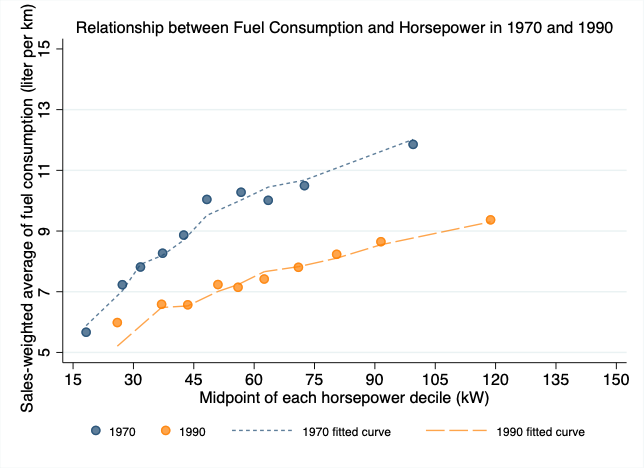
\includegraphics[width = \textwidth]{output/figure/relation_li_hp.png}
\end{figure}

Based on figure \ref{fig:1}, in general, the sales-weighted average fuel consumption increased as the horsepower increased. Comparing with 1970, the sales-weighted average fuel consumption decreased in 1990 in all horsepower decile groups, and the fitted curve was flatter in 1990. We can extrapolate that, controlling for horsepower, the sales-weighted average fuel consumption decreased over time -- cars in the five European markets became more fuel-efficient.

Suppose a social cost of carbon was imposed across Europe in 1991, causing the price of gas to increases across all five markets. This imposed social cost of carbon would disincentivize consumers to buy cars that have a high fuel consumption, or the cars that have a high horsepower, which positively correlates with fuel consumption. As a result, the sales-weighted average fuel consumption of the cars in the high horsepower group would fall in 1991. The fitted curve in 1991 would be flatter than the one in 1990, especially in the tail of the curve.

Please see table \ref{tab:1} for summary statistics of the sales-weighted average of fuel consumption by decile of horsepower in 1970 and 1990.

\begin{table}
\begin{table}[H] \centering
\newcolumntype{C}{>{\centering\arraybackslash}X}

\caption{Sales-weighted average of fuel consumption by decile of horsepower}
\label{tab:1}
{\small
\begin{tabularx}{\textwidth}{lCCCCCC}

\toprule
& \multicolumn{3}{c}{1970} & \multicolumn{3}{c}{1990} \tabularnewline \cmidrule(lr){2-4} \cmidrule(lr){5-7} \addlinespace[-2.5ex] \tabularnewline {Decile} &{Fuel consumption} &{Horsepower range} &{Sales} &{Fuel consumption} &{Horsepower range} &{Sales}  \tabularnewline
\midrule\addlinespace[1.5ex]
1&5.666&13--23.5&814,581&5.985&19--33&2,197,737 \tabularnewline
2&7.232&25--29.5&1,095,414&6.586&34--40&1,556,830 \tabularnewline
3&7.815&30.5--33&769,165&6.569&41--46&1,045,728 \tabularnewline
4&8.270&34--40.5&1,157,252&7.237&48--54&1,024,291 \tabularnewline
5&8.867&41--44&234,318&7.147&55--57&1,042,327 \tabularnewline
6&10.041&45--51.5&495,287&7.419&59--66&944,924 \tabularnewline
7&10.279&53--60.5&285,753&7.806&67--75&470,646 \tabularnewline
8&10.012&61--66&287,505&8.233&76--85&494,383 \tabularnewline
9&10.495&67--78&326,636&8.648&87--96&345,608 \tabularnewline
10&11.855&81--118&133,559&9.369&96.5--141&232,187 \tabularnewline
\bottomrule \addlinespace[1.5ex]

\end{tabularx}
\begin{flushleft}
\footnotesize Fuel consumption represents the sales-weighted average of fuel consumption.
\end{flushleft}
}
\end{table}

\end{table}

\section{Estimation and Causal
Inference}\label{estimation-and-causal-inference}

For each car model $i$, market $j$, and year $t$, construct the outcome variable $(Y_{ijt} = log(S_{ijt}) - log(S_{0ijt})$, where $N_{jt}$ is the number of consumers in market $j$ year $t$, assuming the average size of family is four and each family potentially buys one car or no cars in a given year, $S_{ijt}$ is the market share for car model $i$ in market $j$ year $t$, $S_{0jt}$ is the share of consumers who buy no cars in market $j$ year $t$.

A standard logit demand model: 
\begin{equation*}
U_{cijt} = \beta_c \text{FuelConsumption}_{ijt} + \alpha_c \text{Price}_{ijt} + \zeta_{ijt} + \epsilon_{cijt}
\end{equation*}

where $c$is an index for car consumers, $i$ car model, $j$ market, and $t$ year. $U$ is the indirect utility, as a function of
the car models' average fuel consumption and price. $\zeta_{ijt}$ is the unobservable variables on the year-market-model level.  $\epsilon_{cijt}$ is unobservable variables on the year-market-model-consumer level.

Assume the structural parameters, $\beta$ and $\alpha$, do not
depend on individual consumer (every consumer has the same taste for
fuel consumption and price), $\epsilon_{cijt}$ has type-one extreme
value function, and all consumers who did not buy a car chose the
outside option, which gives zero utility. Then, we can estimate the
structural parameter through the following log-linear model:

\begin{equation} \label{eqn:1}
log(S_{ijt}) - log(S_{0ijt}) = \beta \text{FuelConsumption}_{ijt} + \alpha Price_{ijt} + \zeta_{ijt}
\end{equation}

$\zeta_{ijt}$ is a shock on the demand side.

Table \ref{tab:2} reports the results of this regression. We estimate the coefficient of fuel consumption, $\beta$, to be
$-0.214$. It means that, holding everything else equal, the consumers' indirect utility decreases by $0.214$ unit as the fuel consumption of the car increases by $1$ unit.

\begin{table}[H]
\centering
{
\def\sym#1{\ifmmode^{#1}\else\(^{#1}\)\fi}
\caption{Structural parameters for fuel consumption and price \label{tab:1}}
\begin{tabular*}{\textwidth}{@{\hskip\tabcolsep\extracolsep\fill}l*{4}{c}}
\toprule
                    &\multicolumn{1}{c}{(1)}&\multicolumn{1}{c}{(2)}&\multicolumn{1}{c}{(3)}&\multicolumn{1}{c}{(4)}\\
                    &\multicolumn{1}{c}{Outcome}&\multicolumn{1}{c}{Outcome}&\multicolumn{1}{c}{Outcome}&\multicolumn{1}{c}{Outcome}\\
\midrule
Fuel consumption (liter per km)&      -0.214\sym{***}&      -0.214\sym{***}&      -0.214\sym{**} &      -0.214\sym{***}\\
                    &   (0.00926)         &    (0.0308)         &    (0.0391)         &    (0.0122)         \\
\addlinespace
Price in common currency&  -0.0000578\sym{***}&  -0.0000587\sym{***}&  -0.0000578\sym{**} &  -0.0000578\sym{***}\\
                    &(0.00000421)         & (0.0000123)         &(0.00000936)         &(0.00000854)         \\
\addlinespace
Constant            &      -5.067\sym{***}&      -5.053\sym{***}&      -5.067\sym{***}&      -5.067\sym{***}\\
                    &    (0.0784)         &     (0.295)         &     (0.317)         &    (0.0884)         \\
\midrule
Observations        &        7679         &        7653         &        7679         &        7679         \\
Fixed effects       &        None         &        None         &        None         &        None         \\
Standard errors     &Non-clustered robust         &Clustered on model         &Clustered on market         &Clustered on year         \\
\bottomrule
\multicolumn{5}{l}{\footnotesize Standard errors in parentheses}\\
\multicolumn{5}{l}{\footnotesize \sym{*} \(p<0.05\), \sym{**} \(p<0.01\), \sym{***} \(p<0.001\)}\\
\end{tabular*}
}

\end{table}

Table \ref{tab:2} also reports the standard errors under different specifications.  Column (1) reports the heteroskedastic robust standard errors and column (2) the standard errors clustered on car models.  To cluster the standard errors on car models, we assume the observations are independent across car models but not necessarily within each model.  This assumption is not entirely plausible because different car models may be similar in design.  Other specifications of standard errors are less convincing.  For instance, to cluster on years, we need to assume that observations are independent across years.  But it is reasonable to assume that consumers' preferences are auto-correlated. 

Price is an endogenous variable in model \ref{eqn:1}. Price is correlated with $\zeta_{ijt}$, the demand shock. Assuming the demand shock is observable to manufacturers, then manufacturers would adjust the prices accordingly.

There are two different sources of endogeneity that could bias our estimate of the structural parameter of price.

One source of endogeneity is the un-observalbe features of the car models, markets, or years. For example, consumers may prefer one particular type of car models for reasons other than its fuel consumption or price, but for the models' un-observable features. Denote them as $\phi_i$. Similarly, consumers may experience some market-specific, model-and-year-invariant shock, $\phi_j$, or some year-specifc, model-and-market-invariant shock, $\phi_t$.

We can mitigate this type of endogeneity by including car model, market, and year fixed effects.

\begin{equation} \label{eqn:2}
log(S_{ijt}) - log(S_{0ijt}) = \beta \text{FuelConsumption}_{ijt} + \alpha Price_{ijt} + \zeta_{ijt} + \phi_i + \phi_j + \phi_t
\end{equation}

Controlling for car model, market, and year fixed effects, we report the coefficients of fuel consumption and price in table \ref{tab:3}

\begin{table}[H]
\centering
{
\def\sym#1{\ifmmode^{#1}\else\(^{#1}\)\fi}
\caption{Structural parameters for fuel consumption and price (added fixed effects) \label{tab:2}}
\begin{tabular*}{\textwidth}{@{\hskip\tabcolsep\extracolsep\fill}l*{4}{c}}
\toprule
                    &\multicolumn{1}{c}{(1)}&\multicolumn{1}{c}{(2)}&\multicolumn{1}{c}{(3)}&\multicolumn{1}{c}{(4)}\\
                    &\multicolumn{1}{c}{Outcome}&\multicolumn{1}{c}{Outcome}&\multicolumn{1}{c}{Outcome}&\multicolumn{1}{c}{Outcome}\\
\midrule
Fuel consumption (liter per km)&      -0.138\sym{***}&      -0.138\sym{***}&      -0.138\sym{*}  &      -0.138\sym{***}\\
                    &    (0.0178)         &    (0.0351)         &    (0.0300)         &    (0.0148)         \\
\addlinespace
Price in common currency&   -0.000103\sym{***}&   -0.000103\sym{***}&   -0.000103\sym{**} &   -0.000103\sym{***}\\
                    & (0.0000102)         & (0.0000255)         & (0.0000145)         & (0.0000187)         \\
\addlinespace
Constant            &      -4.610\sym{***}&      -4.610\sym{***}&      -4.610\sym{***}&      -4.610\sym{***}\\
                    &     (0.217)         &     (0.360)         &     (0.378)         &     (0.208)         \\
\midrule
Observations        &        7653         &        7653         &        7653         &        7653         \\
Fixed effects       &car model, market, and year         &car model, market, and year         &car model, market, and year         &car model, market, and year         \\
Standard errors     &                     &Clustered on model         &Clustered on market         &Clustered on year         \\
\bottomrule
\multicolumn{5}{l}{\footnotesize Standard errors in parentheses}\\
\multicolumn{5}{l}{\footnotesize \sym{*} \(p<0.05\), \sym{**} \(p<0.01\), \sym{***} \(p<0.001\)}\\
\end{tabular*}
}

\end{table}

Another source of endogenity comes from the market structure. For example, if the car markets in the five European countries are not perfectly competitive, there still exists potential correlation between price and demand shock even if we controlled for all fixed effects.

To mitigate the second source of endogenity, we need to use an instrument variable for price. One candidate of the instrument variable is the transportation cost: the cost needed to transport cars from their manufacturing locations to their markets. This is because the transportation cost is the supply-shifter that does not shift the demand: it's uncorrelated with the demand shock $\zeta_{ijt}$.

\end{document}
